\documentclass{abnt}
\usepackage[utf8]{inputenc}
\usepackage[english,brazilian]{babel}
\usepackage{hyperref}
\usepackage{url}
\usepackage{indentfirst}
\usepackage{blindtext}
\hypersetup{%
    pdfborder = {0 0 0}
}
\usepackage{graphicx}
\graphicspath{{./imagens/}}
\usepackage{placeins}

\usepackage{longtable}
\usepackage{floatpag}% http://ctan.org/pkg/floatpag
\usepackage{fancyhdr}% http://ctan.org/pkg/fancyhdr
\usepackage[absolute]{textpos}

\usepackage[final]{pdfpages}
\usepackage{pdflscape}
\usepackage{rotating}

\usepackage{color, colortbl}
\definecolor{cNaoImplementado}{rgb}{0.80,0.80,0.80}
\definecolor{cImplementado}{rgb}{0,0.8,0} 
\definecolor{cUserSprint}{rgb}{0.25,0.41,0.88} 
\begin{document}

\autor{ Juliano Rodovalho Macedo \\ Rafael Tavares Amorim \\ Wolmir L. F. Nemitz}

\titulo{Entrega 4: Gestão de Disponibilidade \\ Versão 3.0}

\instituicao{Universidade Federal do Pampa \par Engenharia da Software \par Resolução de Problemas V}

\local{Alegrete - Rio Grande do Sul, Brasil}

\data{04 de Outubro de 2012}

\capa

\folhaderosto

\tableofcontents

\listoffigures


\chapter{Introdução}

	Este relatório tem por finalidade apresentar a fundamentação teórica e tecnológica utilizada no quarto \emph{sprint}, o nosso Product Backlog completo e atualizado, 
	o Sprint Backlog munido de nossas especificações de engenharia juntamente com o detalhamento da solução, e por fim, o link de referência visando o acesso ao sistema.

	\section{Metodologia Ágil}
	
		Metodologia ágil é um famoso conjunto de metodologias de desenvolvimento de software, 
		com foco na mitigação dos riscos, esta metodologia aposta em pequenos ciclos iterativos de desenvolvimento de software,
		onde ocorre a repetição de cada tarefa comum em um processo de software, ou seja, em cada ciclo realiza-se analise, projeto,
		implementação e testes, referentes aquele módulo, desta forma busca-se à capacidade real de implantar um nova versão 
		do sistema ao final de cada ciclo;  Antes de iniciar-se uma nova iteração a equipe responsável por todo o projeto é reunida 
		e reavalia-se as características, metas e prioridades do projeto como um todo, para que estas sejam aplicadas no próximo ciclo.
		
		Os modelos ágeis são hoje a principal alternativa as metodologias tradicionais de desenvolvimento de software, 
		as quais apresentam diversos problemas estruturais que comprometem a maioria dos projetos, 
		baseados nas necessidades atuais do mercado de software.
	
	\section{Scrum}
	
		\subsection{Visão Geral}
		
			O \emph{scrum} é uma metodologia ágil de desenvolvimento de software, embora muitos consideram-no como um framework ágil, 
			o seus maior objetivo é agilizar o processo de desenvolvimento de software com pequenas entregas ao cliente de forma iterativa
			visando agregar-se valor ao produto a cada ciclo(iteração) . Em sua existem três papéis neste processo, são eles: \emph{Product Owner, Scrum Master, Team}.
		
		\subsection{Papéis}
		
			O \emph{Product Owner} é um papel muito importante no \emph{scrum}, cabe a ele definir quais funcionalidades devem ou
			não existir no sistema por meio de \emph{user stories} e também definir a prioridade delas. Este pa\texttt{}pel também
			trata de aprovar ou rejeitar o trabalho realizado e dizer se foi realizado como esperado.
			
			O \emph{scrum master} tem papel de manter a produtividade da equipe, facilitando o processo de \emph{scrum} e resolver impedimentos
			no decorrer do \emph{sprint}. Ele ajuda o time a se manter organizado e certificar que as regras do processo estão sendo
			seguidas corretamente. O \emph{scrum master} não dita o que o time deve fazer mas sim ajuda o time se manter autônomo,
			organizado e com uma boa produtividade. 
			
			O \emph{team} tem papel de transformar os itens de \emph{backlog} em produtos que serão entregues de forma incremental em cada
			sprint. Cabe ao time ter autonomia própria para se organizar e trabalhar de forma de colaborativa ajudando uns aos
			outros sem a necessidade de existência de um "chefe" para dizer o que deve ser feito.
		
		\subsection{Processo}
		
			O processo de \emph{scrum} é trabalhado em cima de vários ciclos chamados de \emph{sprint}, que possuem um tempo fixo, geralmente de
			1 a 4 semanas. Para cada \emph{sprint} é realizado a escolha de \emph{user stories} que estão no \emph{product backlog}. No \emph{product backlog} temos uma lista priorizada 
			pelo \emph{product owner} das funcionalidades desejadas do projeto, e parte desta lista irá forma o \emph{sprint backlog}. É uma coleção de \emph{user stories}.
			
			Em um ciclo, o time irá realizar o \emph{sprint backlog} que contêm os itens de \emph{backlog} que o time concordou 
			completar em um ciclo de \emph{sprint}, cada item de \emph{backlog} é quebrado em tarefas, atribuídas para equipe e estimado o tempo de realização.
			
					
			O \emph{backlog item} ou também conhecido como \emph{user story} é um recurso/funcionalidade desejada no sistema que vão compor o
			\emph{product backlog}. Uma \emph{user story} usualmente é composta por um ator do sistema e a ação para alcançar determinado
			objetivo. Exemplos: 
				\begin{itemize}
					\item Como um usuário Eu posso realizar a ação para alcançar determinado objetivo
					\item Como um cliente, eu posso criar um perfil no sistema
					\item Como um cliente, eu posso escolher um usuário e senha
					\item Como um administrador, eu posso bloquear contas de clientes
				\end{itemize}
					 
					
			No \emph{sprint planning}, a equipe decidirá quais \emph{backlog itens} irão para o \emph{sprint backlog}. Depois da priorização das \emph{user
			stories} pelo \emph{product owner}, a equipe seleciona o item do topo do \emph{product backlog}, o qual tem maior prioridade, para a
			discussão e criação das tarefas necessárias para entrega do item. Então as tarefas são atribuídas e estimadas em
			tempo, este processo é repetido até que o time decida que não há possibilidade de realização de mais itens.
			
			Com a ajuda do\emph{Burndown} que é um gráfico que oferece uma forma poderosa que podemos analisar o andamento do projeto. Podemos estimar a velocidade de andamento do time, atrasos e tempo de 
			execução de cada \emph{user story}.
			
			Por meio de um reunião diariamente, podemos também verificar impedimentos que podem afetar a produtividade da equipe, conhecida como \emph{daily meeting}, 
			é uma reunião com duração aproximada de 15 minutos,	conduzida pelo \emph{scrum master} e tem como foco 3 perguntas para todo membro da equipe:
				\begin{itemize}
					\item O que eu fiz ontem?
					\item O que eu estou fazendo hoje?
					\item O que está me impedindo de fazer?
				\end{itemize}
			
			Apesar da reunião ser conduzida pelo scrum master, cada membro deve responder para o time inteiro e não somente para o
			\emph{scrum master}, todos devem estar de pé na reunião e falar somente quando for perguntado pelo \emph{scrum master}. No final da
			reunião é discutido por todos soluções caso haja algum impedimento.
			
			No final de um \emph{sprint}, ocorre uma reunião informal, chamada \emph{sprint review} que tem intuito de demonstrar o que foi 
			realizado no sprint com a presença da equipe, \emph{scrum master}, \emph{product owner} e stakeholders. Também é feita a reunião chamada \emph{sprint retrospective}
			que é uma reunião da equipe que tem objetivo de discutir se o \emph{sprint} foi realizado com sucesso ou se é necessário melhorias.
			
			Um projeto em \emph{scrum} pode ser parado a qualquer momento, as vezes o cliente percebe que as funcionalidade implementadas já foram
			suficientes e atendem a necessidade atual assim não dispersando dinheiro em funcionalidade que talvez nunca seriam utilizadas.
			
			As informações desta seção foram retiradas da referência \cite{SCRUMEPF}.
	
		%Importação errada, arrumar futuramente
		%\setlength{\arrayrulewidth}{1.5pt}
\begin{landscape}
	\chapter{Product Backlog Atualizado - Sprint 04}
		% Table generated by Excel2LaTeX from sheet 'Plan1'
		\begin{longtable}{|p{0.5in}|p{6in}|c|c|}
		
		\hline
		  {\bf ID} & {\bf Users Stories} & {\bf Tempo Previsto} & {\bf Status} \\
	
		\hline \rowcolor{cImplementado}
		         1 & Como professor, eu quero decidir quais compromissos são públicos ou privados para manter sigilo. &         10 & Implementado \\
		
		\hline \rowcolor{cImplementado}
		         2 & Como professor, eu quero a partir de uma disciplina cadastrar um plano de ensino com o programa e as bibliografias suplementares para as disciplinas que eu vou ministrar. &         40 & Implementado \\
		
		\hline \rowcolor{cImplementado}
		         3 & Como professor, eu quero cadastrar meus compromissos no sistema para que todos saibam quando não posso agendar outro compromisso. &         40 & Implementado \\
		\hline \rowcolor{cNaoImplementado}
		         4 & Como secretária eu desejo acessar as informações de horários e disponibilidade de cada sala do campus.  &         20 & Não Implementado \\
		
		\hline  \rowcolor{cNaoImplementado}
		         5 & Como usuário, eu quero poder pedir minha senha por email para que eu possa recuperar caso eu tenha perdido. &         10 & Não Implementado \\
		
		\hline \rowcolor{cNaoImplementado}
		         6 & Como professor, eu quero navegar por todas as disciplinas disponíveis para visualizar as disciplinas que tenho interesse.  &         40 & Não Implementado \\
		
		\hline \rowcolor{cNaoImplementado}
		         7 & Como professor, eu quero ver a disponibilidade dos equipamentos como caixa de som, projetores e outros para poder fazer um agendamento. &         40 & Não Implementado \\
		
		\hline \rowcolor{cNaoImplementado}
		         8 & Como professor, eu quero visualizar minha grade horária de aulas para saber os horários que tenho que dar aula. &         40 & Não Implementado \\
		
		\hline \rowcolor{cImplementado}
		         9 & Como professor, eu quero informar os dias que estarei na unipampa para que os outros possam me encontrar para assuntos urgentes.  &         20 & Implementado \\
		
		\hline	\rowcolor{cImplementado}
		        10 & Como professor, eu quero informar meu horário disponível para as aulas. &         40 & Implementado \\
		
		\hline	\rowcolor{cUserSprint}
				11 & Como professor, eu quero informar minhas disciplinas de preferência. & 			60 & Não Implementado \\	
		
		\hline	\rowcolor{cNaoImplementado}
				12 & Como professor, eu quero informar minha área de formação para que o coordenador possa montar a grade de aulas de acordo com os dados que informei. & 60 & Não Implementado \\
		
		\hline	\rowcolor{cNaoImplementado}
		        13 & Como professor, eu quero agendar reuniões com os outros professores em horários que não choquem com compromissos deles e esperar que eles aceitem.  &         30 & Não Implementado \\
		
		\hline \rowcolor{cUserSprint}
		        14 & Como usuário, eu quero ter um usuário e senha para que eu possa acessar minha conta pessoal no sistema. &         30 & Não Implementado \\
		
		\hline \rowcolor{cNaoImplementado}
		        15 & Como secretária, eu quero visualizar salas e equipamentos que estão alocados para quem e quando.  &         20 & Não Implementado \\
		
		\hline \rowcolor{cNaoImplementado}
		        16 & Como secretária, eu quero cadastrar os equipamentos de uso da instituição para que os professores possam ver sua disponibilidade.  &         40 & Não Implementado \\
		
		\hline \rowcolor{cNaoImplementado}
		        17 & Como secretária, eu quero cadastrar as salas, com seu tipo e capacidade para que o coordenador possa vê-las podendo organizar as ofertas das disciplinas. &         40 & Não Implementado \\
		
		\hline \rowcolor{cNaoImplementado}
		        18 & Como coordenador, eu quero cadastrar as disciplinas juntamente com sua descrição, ementa, pré-requisitos e sua necessidade de sala que poderão ser ofertadas no sistema e para que os professores possam escolher suas preferidas. &         40 & Não Implementado \\
		
		\hline \rowcolor{cNaoImplementado}
		        19 & Como coordenador, eu quero ver o perfil de cada professor para que eu possa avaliar suas áreas.  &         10 & Não Implementado \\
		
		\hline \rowcolor{cUserSprint}
		        20 & Como coordenador, eu quero alocar disciplinas em horários específicos, alocar os professores e salas para elas assim possibilitando sua oferta.  &         60 & Não Implementado \\
		
		\hline \rowcolor{cUserSprint}
		        21 & Como professor, eu quero me registrar no sistema para que eu possa fornecer meus dados ao coordenador. &         30 & Não Implementado \\
		
		\hline \rowcolor{cNaoImplementado}
		        22 & Refatorar formulário de cadastro de disciplinas e salas/tipos com intuito de melhorar a visibilidade e aparência.  &         40 & Não Implementado \\
		
		\hline \rowcolor{cNaoImplementado}
		        23 & Refatorar o DB de disciplinas separando curso, turma e campus em objetos diferentes e não atributos. &         30 & Não Implementado \\
		
		\hline \rowcolor{cNaoImplementado}
		        24 & Refatorar o DB de disciplina para receber pré-requisitos em forma de n objetos invés de campo texto. &         20 & Não Implementado \\
		
		\hline \rowcolor{cNaoImplementado}
				Defeito \#336 & Correção da marcação do Campo Obrigatório no form de disciplinas.  &          5 & Não Implementado \\
		
		\hline \rowcolor{cImplementado}
				Defeito \#399  & Correção da adição desconhecida da string (u'') ao editar um compromisso, no form de compromisso no área de professor. &          1 & Implementado \\
		
		\hline
		\caption{Product Backlog}
		\end{longtable}
		
		\textbf{Tabela de Legenda} \\
		\begin{tabular}{|c|c|}
		\hline 
		{\bf Cor} & {\bf Legenda} \\
		\hline \textcolor{cImplementado}{\begin{huge} $\bullet$ \end{huge}} & Implementado \\
%		\hline \textcolor{fblueParcialmentImp}{\begin{huge} $\bullet$ \end{huge}} & Parcialmente Implementado \\
		\hline \textcolor{cNaoImplementado}{\begin{huge} $\bullet$ \end{huge}} & Não Implementado \\
		\hline \textcolor{cUserSprint}{\begin{huge} $\bullet$ \end{huge}} & User Stories do Sprint Atual \\
		\hline
		\end{tabular}

		Data de geração: \today
		

\end{landscape}

		

\clearpage

\chapter{Sprint}
	
		Esta seção aborda as informações sobre o Sprint IV, demonstrando o nosso \emph{Sprint Backlog} logo a baixo. Os diagramas de casos de uso e classes para cada \emph{User Story} está disponível nas seções seguintes.
	
			
		\section{Funcionalidades - Versão 3.0}
		
			As funcionalidades entregues nesta versão são:
		
			\begin{itemize} 
			\item Crud Disciplinas de Preferência:
			\subitem Informar disciplinas de preferência
			\subitem Visualizar disciplinas de preferência
			\subitem Editar disciplinas de preferência
			\subitem Remover disciplinas de preferência
			
			\item Oferta de Disciplinas
			\subitem Criar grade da turma
			\subitem Associar par Professor-Disciplina
			\subitem Remover disciplina ofertada
			
			\item Registrar no sistema
			\subitem Cadastrar no sistema
			
			\item Login e Logout 
			\subitem Realizar Login no sistema
			\subitem Realizar Logout no sistema
			
			\end{itemize}
			
	\clearpage
	\section{User Story 1}
	
		\begin{itemize}
			\item Como professor, eu quero informar minhas disciplinas de preferência.
		\end{itemize}
		
		Status: Implementado
		
		\subsection{Mockup}
		
		\begin{figure}[h]
					\begin{center}
						 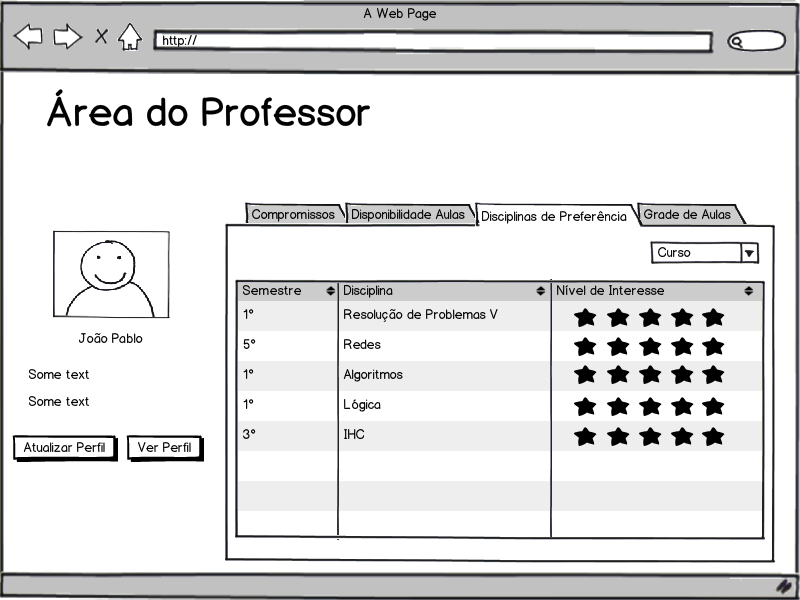
\includegraphics[width=400px]{telaProfessorDisciplinas}
						 \caption{Mockup - Informar interesse em disciplina}
						 %\label{fig:CasoUsoDiasAusencia}
					\end{center}
				\end{figure}
		
		\subsection{Diagramas de Caso de Uso}	
		\begin{figure}[h]
			\begin{center}
				 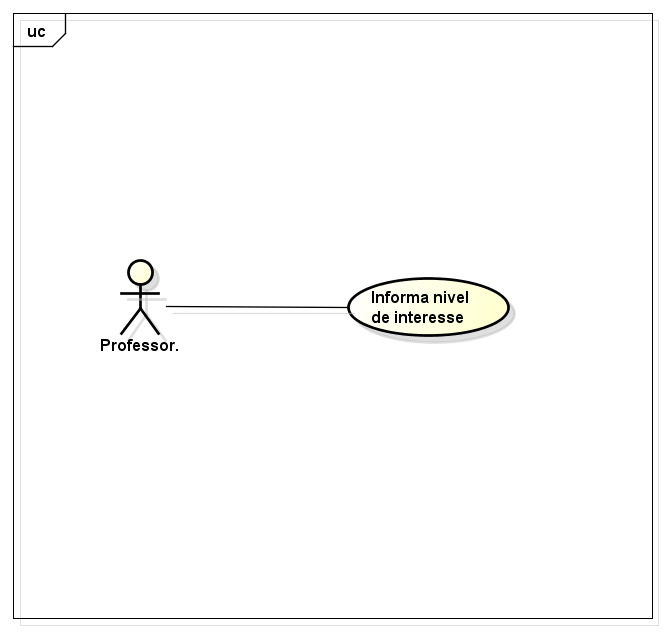
\includegraphics[width=400px]{casoUsoInformarInteresseDisciplina}
				 \caption{Diagrama de Caso de Uso - Informar interesse em disciplina}
				 %\label{fig:CasoUsoDiasAusencia}
			\end{center}
		\end{figure}
		
		\FloatBarrier
		
		\subsection{Caso de Uso Expandido - Informar Nível de Interesse em Disciplina}
		\begin{figure}[h]
			\begin{center}
				 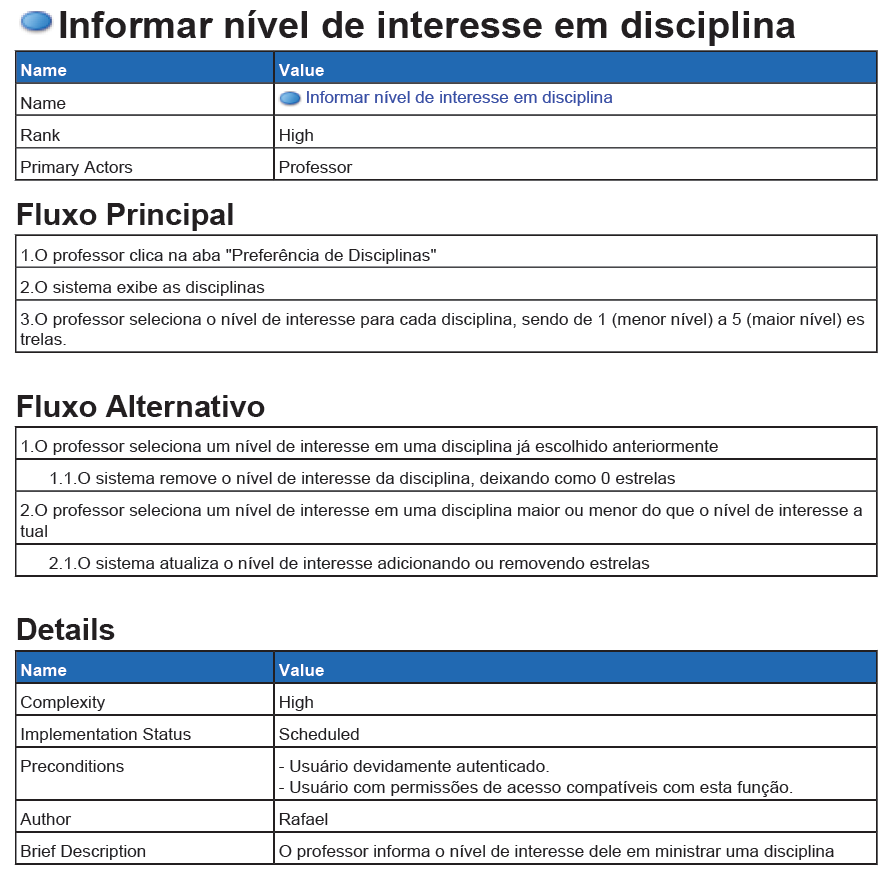
\includegraphics[width=450px]{casoUsoInformarNivelInteresseDisciplina}
				 \caption{Caso de Uso Expandido - Informar Nível de Interesse em Disciplina}
				 %\label{fig:CasoUsoDisponibilidadeHorario}
			\end{center}
		\end{figure}
		\FloatBarrier
		
		
		\subsection{Diagramas de Sequência}
		\begin{figure}[h]
					\begin{center}
						 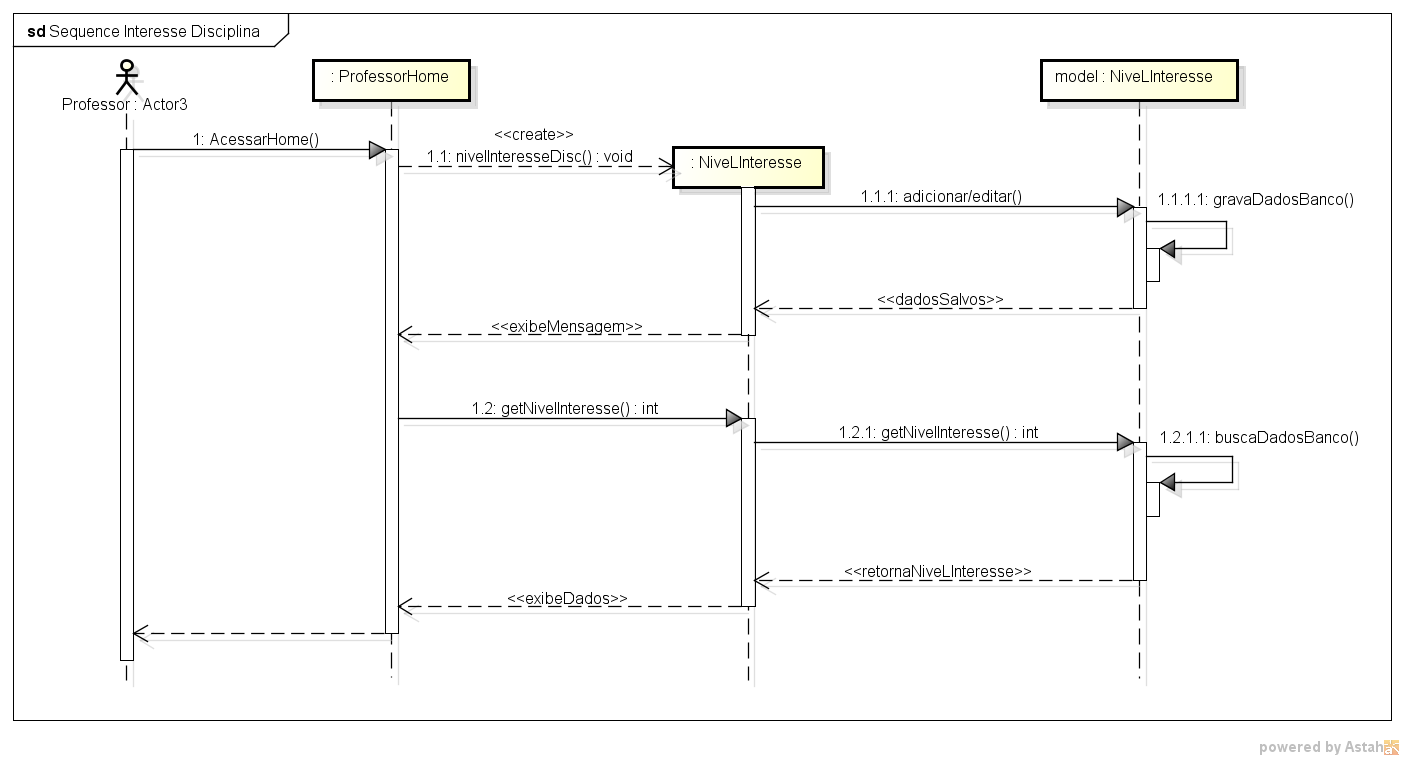
\includegraphics[width=400px]{SequenceInteresseDisciplina}
						 \caption{Diagrama de Sequência - Informar interesse em disciplina}
						 %\label{fig:CasoUsoDiasAusencia}
					\end{center}
				\end{figure}
		
				\FloatBarrier
		
	\clearpage	
	\section{User Story 2}
	 
		\begin{itemize}
			\item Como usuário, eu quero ter um usuário e senha para que eu possa acessar minha conta pessoal no sistema.
		\end{itemize}
		
		Status: Implementado
			
			
	\clearpage
	\section{User Story 3}

		\begin{itemize}
			\item Como coordenador, eu quero alocar disciplinas em horários específicos, alocar os professores e salas para elas assim possibilitando sua oferta.
		\end{itemize}
		
		Status: Não Implementado
		
			\subsection{Mockup}
				
				\begin{figure}[h]
							\begin{center}
								 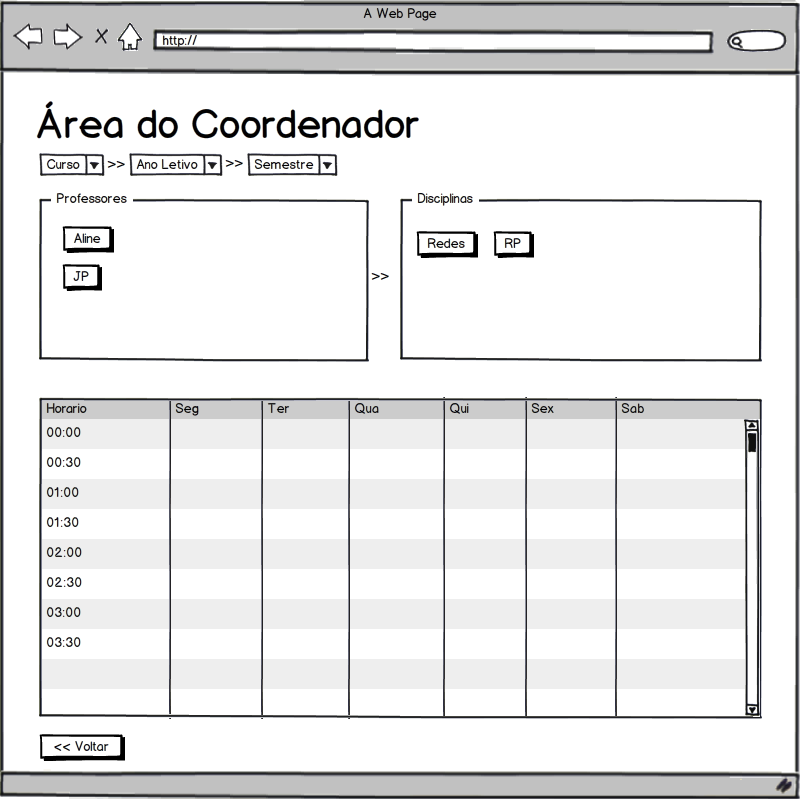
\includegraphics[width=400px]{telaCoordenadorMontarGrade}
								 \caption{Mockup - Montar Grade de Aulas}
								 %\label{fig:CasoUsoDiasAusencia}
							\end{center}
						\end{figure}
			\clearpage
		\subsection{Diagramas de Caso de Uso}
			\begin{figure}[h]
				\begin{center}
				 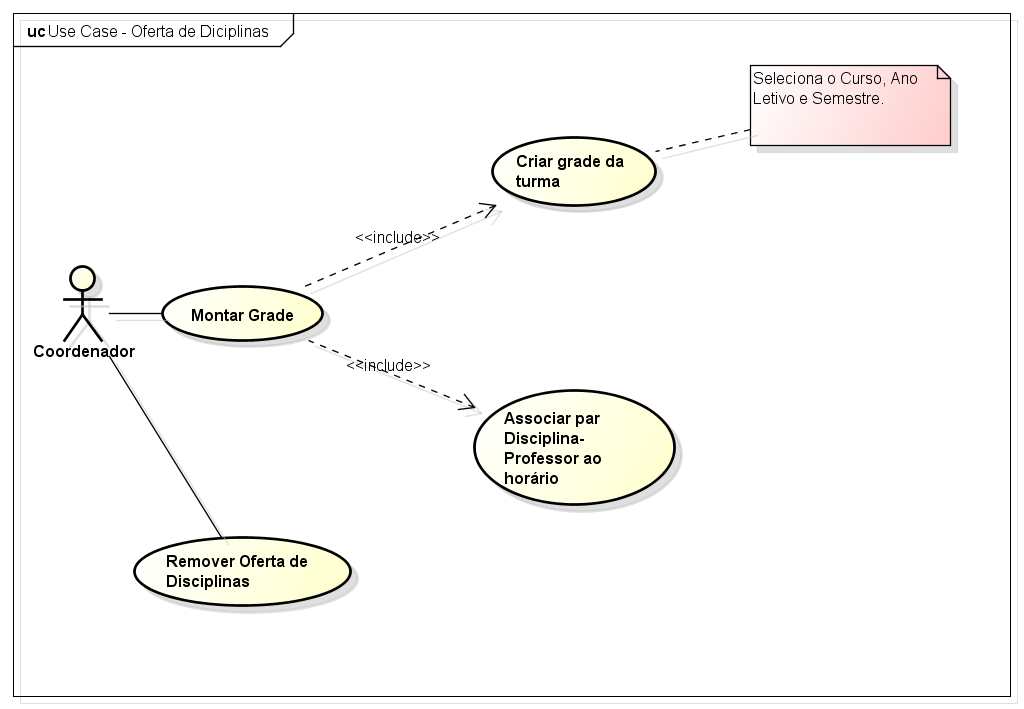
\includegraphics[width=450px]{casoUsoOfertaDisciplinas}
				 \caption{Diagrama de Caso de Uso - Montar Grade de Aulas}
				 %\label{fig:CasoUsoUserStory3}
				\end{center}
			\end{figure}
			\FloatBarrier
			%\clearpage
			\subsection{Caso de Uso Expandido - Oferta de Disciplinas}
		% referência:  http://ask.metafilter.com/32225/Including-PDF-figures-in-a-LaTeX-document
		\begin{figure}[h]
			\begin{center}
				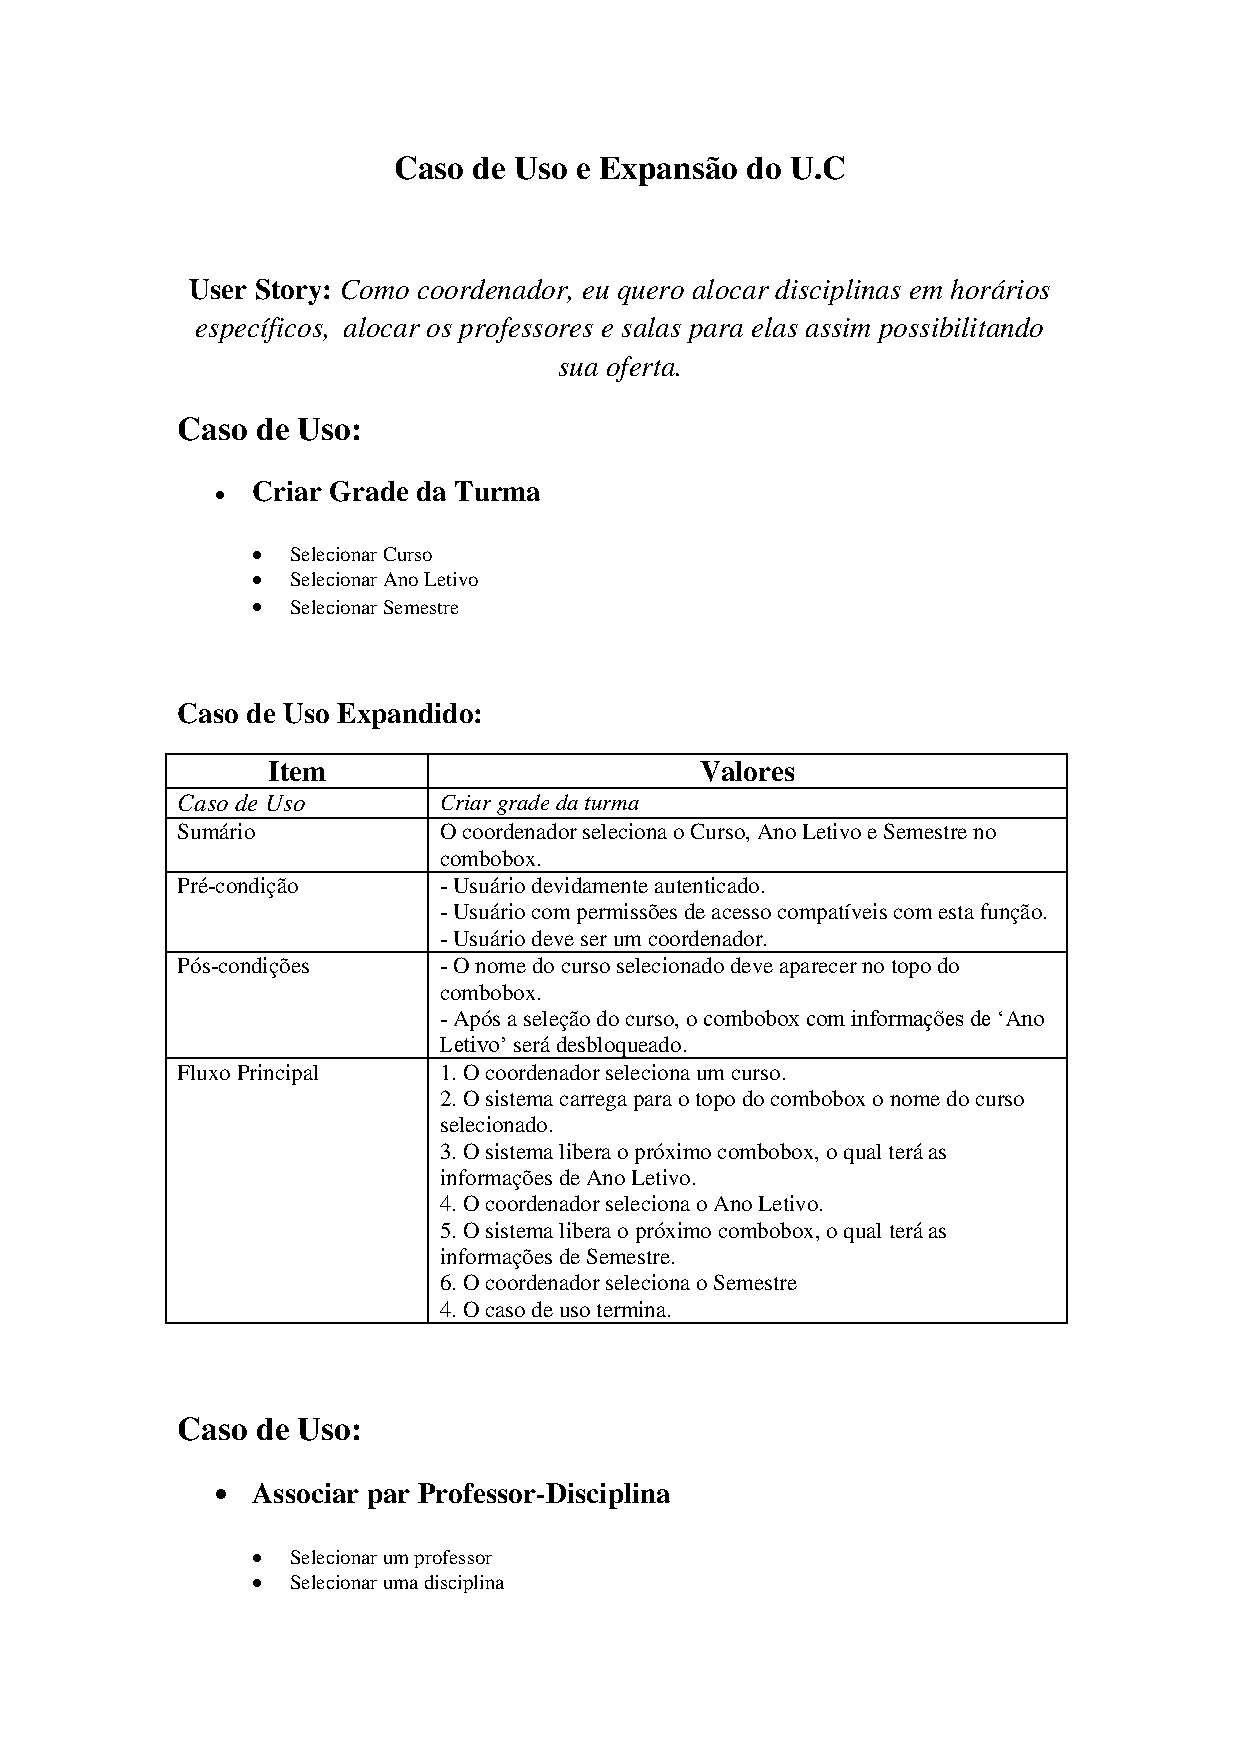
\includegraphics[bb=1.0in 1.0in 7.5in 10in page=1]{ExpansaoU_C_OfertaDisciplinas.pdf}
				 \caption{Caso de Uso Expandido - Oferta de Disciplinas}
			\end{center}
		\end{figure}
		\begin{figure}[h]
			\begin{center}
				\includegraphics[bb=1.0in 1.0in 7.5in 10in,page=2]{ExpansaoU_C_OfertaDisciplinas.pdf}
				 \caption{Caso de Uso Expandido - Oferta de Disciplinas}
			\end{center}
		\end{figure}
		\FloatBarrier

			
	\clearpage
		\section{User Story 4}
	
			\begin{itemize}
				\item Como professor, eu quero me registrar no sistema para que eu possa fornecer meus dados ao coordenador.
			\end{itemize}
			
			Status: Implementado
		
	\clearpage
	
		\section{Diagrama de Classes}
		
			A figura \ref{fig:DiagramaClassesModelo} na próxima página mostra o diagrama de classes da solução implementada para as \emph{user stories} do \emph{sprint}. As classes e atributos referente ao sprint estão em um tom vermelho.
			
					 \begin{landscape}
					 			\begin{figure}[htp]
					 				\begin{center}
					 					 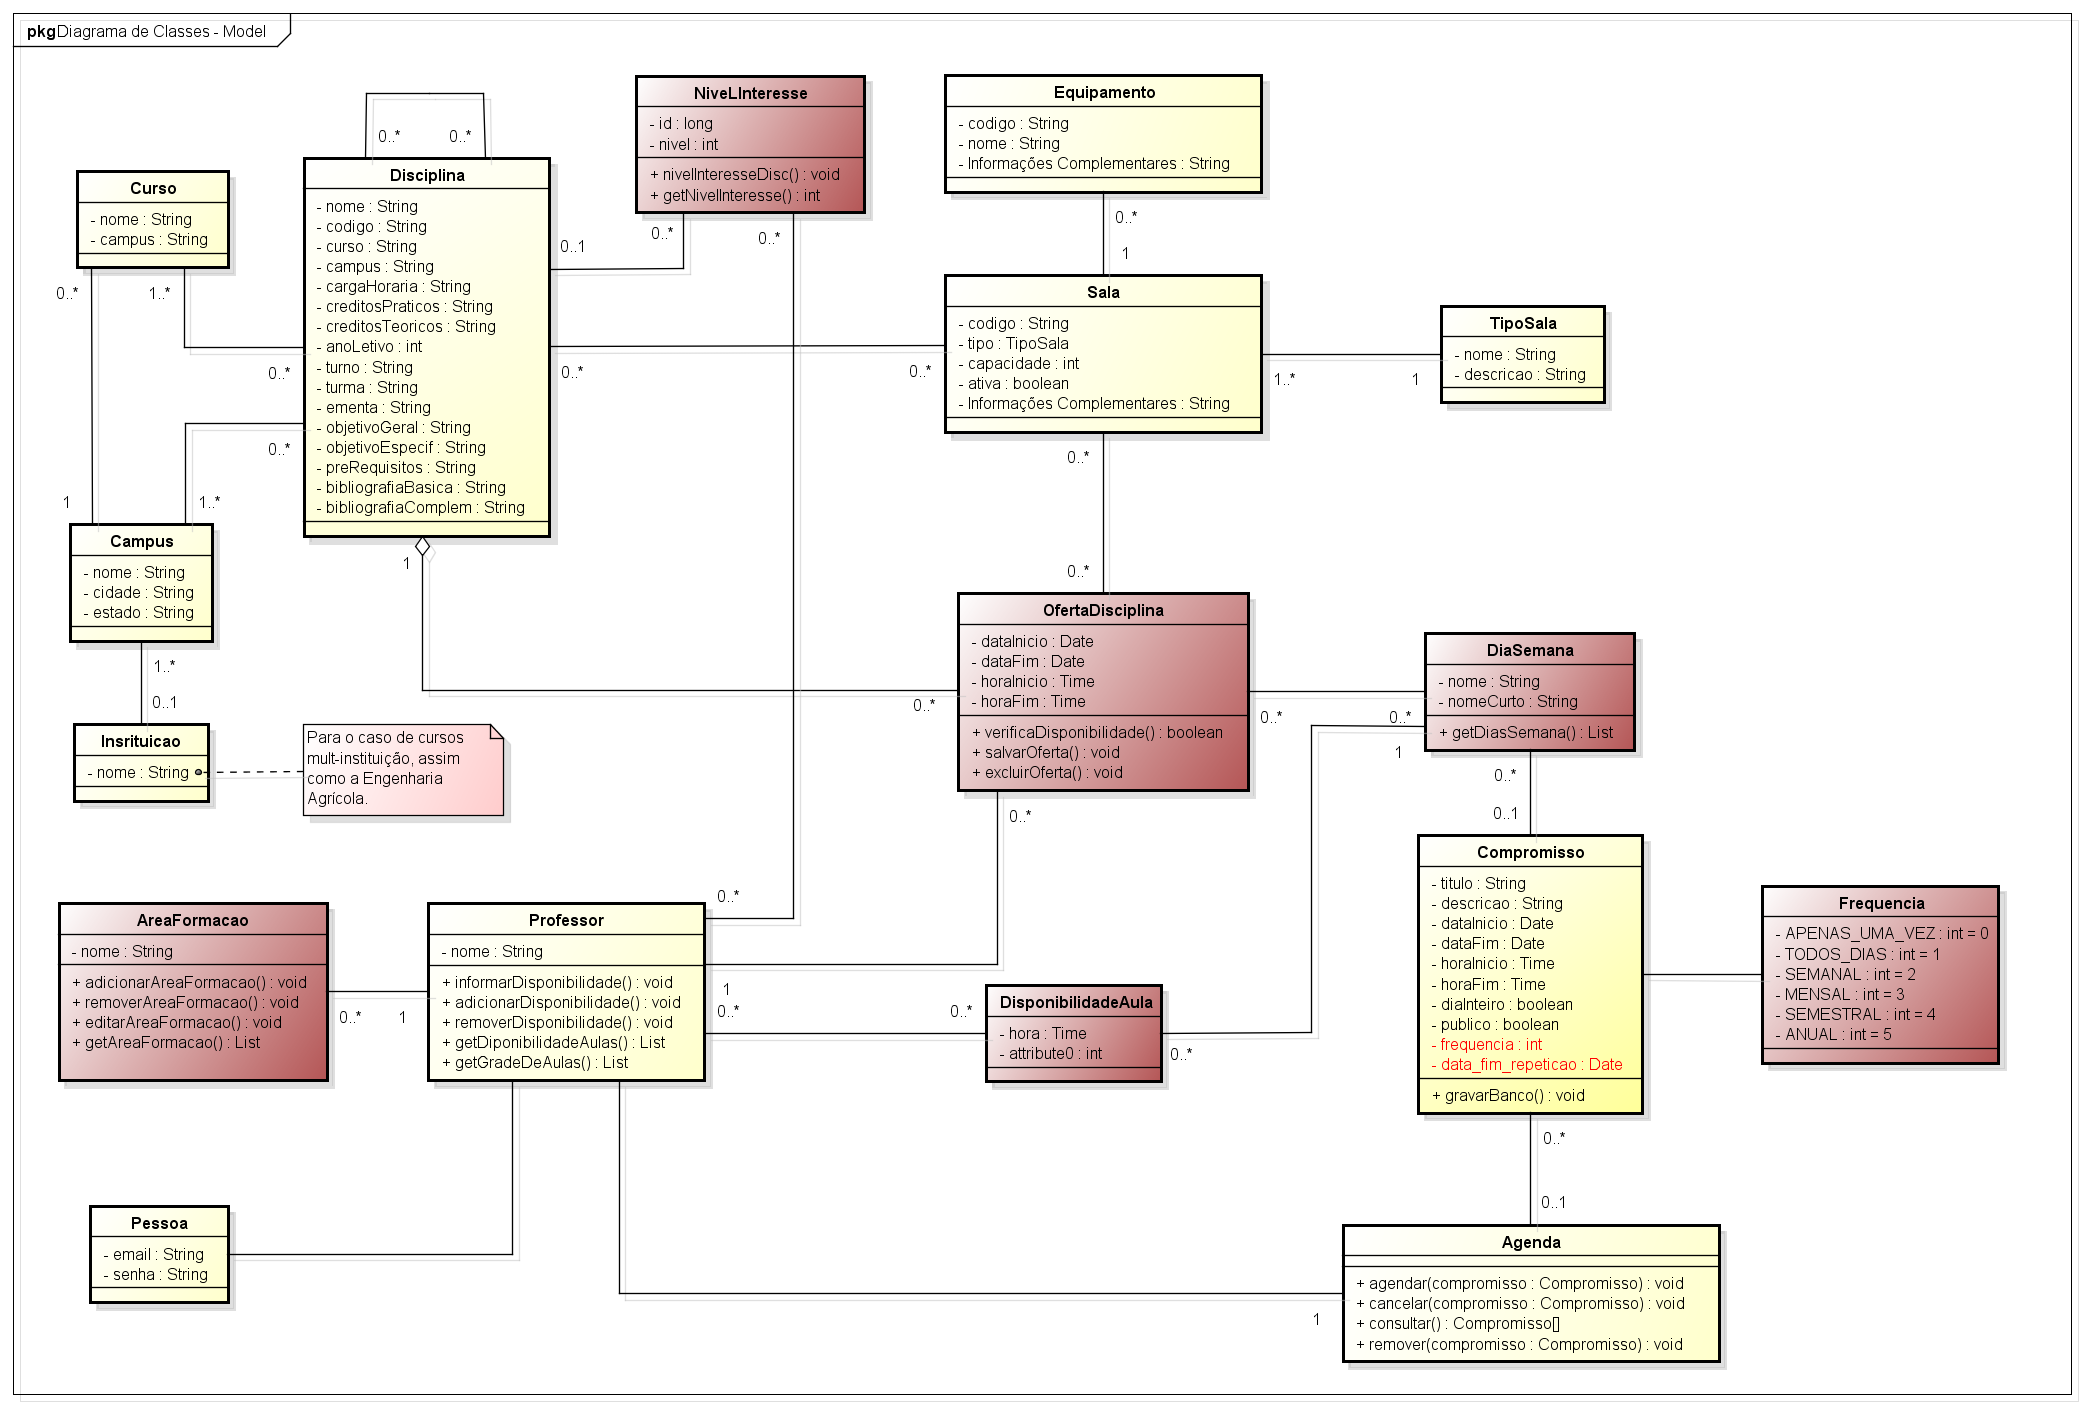
\includegraphics[width=600px]{DiagramaClassesModelo}
					 					 \caption{Diagrama de Classes Modelo}
					 					 \label{fig:DiagramaClassesModelo}
					 				\end{center}
					 			\end{figure}
					 			%\FloatBarrier
					 		\end{landscape}
			
	
		\section{Casos de Teste}
		
		 Por limitação de exportação das descrições da ferramenta, os casos de teste podem ser visto no link \url{http://chicago1.vsnetwork.net:8080/klaros-web/pages/login.seam} com usuário \emph{professor} e senha \emph{professor}
		 
		 Os casos de teste estão agrupados em 2 suites de teste:
		 \begin{itemize}
		 \item TS00006 - Preferência de Disciplinas
		 \item TS00007 - Montar Grade
		 \end{itemize}
		 

		 		 
\clearpage
	\section{Acesso ao Sistema}
			De acordo com o planejamento construído no primeiro \emph{sprint}, o qual definimos nossa infraestrutura de desenvolvimento, 
			o sistema esta em integração contínua com o servidor de testes on-line, contendo todas as funcionalidades da versão 2.0 agora incrementadas para a versão 3.0, 
			podendo ser acessado a partir da seguinte url:
		
			\url{http://chicago1.vsnetwork.net/}
			
			
			

	\section{Acesso às Ferramentas}
		
		O código fonte do projeto pode ser acessado em nosso repositório do github\cite{GITHUB} através da url: \url{https://github.com/dextervip/rpv}. 
		
		As construções automatizadas do jenkins podem ser acessadas através da url: \url{http://chicago2.vsnetwork.net:8080/job/RPV}.

	\clearpage

	%Referências Bibliograficas
	\nocite{*}
	\bibliographystyle{abnt-num}
	%\bibliographystyle{plain}		
	\bibliography{bibliografia}		

\end{document}